\documentclass[11pt,a4paper]{article}
\usepackage[margin=23mm,headheight=15pt]{geometry}
\usepackage{microtype,booktabs,tabularx,array,xcolor,hyperref,fancyhdr,tikz,enumitem,amsmath}
\usetikzlibrary{arrows.meta,positioning,fit,backgrounds}
\definecolor{navy}{HTML}{15324D}
\definecolor{teal}{HTML}{087E83}
\definecolor{pale}{HTML}{ECF5F5}
\definecolor{graytext}{HTML}{526474}
\hypersetup{colorlinks=true,urlcolor=teal,linkcolor=teal}
\pagestyle{fancy}\fancyhf{}\lhead{\small IT457 \quad | \quad WEEK 2 PROGRESS REPORT}\rhead{\small COWIN CASE STUDY}\cfoot{\thepage}\renewcommand{\headrulewidth}{0.4pt}
\setlength{\parindent}{0pt}\setlength{\parskip}{6pt}
\setlist[itemize]{leftmargin=*,nosep,topsep=3pt}\setlist[enumerate]{leftmargin=*,nosep,topsep=3pt}
\newcommand{\sectionline}[1]{\section*{\color{navy}#1}}
\newcolumntype{Y}{>{\raggedright\arraybackslash}X}
\begin{document}
\thispagestyle{empty}
{\color{teal}\large IT457 \ / \ CLOUD COMPUTING}\par\vspace{10mm}
{\color{navy}\LARGE\bfseries Week 2 Progress Report}\par\vspace{3mm}
{\Large CoWIN case study: high availability and failover}\par\vspace{5mm}
\textcolor{graytext}{High-level architecture, PoC plan and team work distribution}\par
\vspace{8mm}\hrule\vspace{7mm}
\begin{tabularx}{\textwidth}{@{}lY@{}}
\textbf{Project theme} & Government and public digital platforms \\
\textbf{Practical focus} & Two-zone cloud proof of concept (PoC) \\
\textbf{Report stage} & Week 2 design and implementation planning \\
\end{tabularx}
\par\vspace{8mm}
\textbf{Project team}\par
\begin{tabularx}{\textwidth}{@{}Yl@{}}\toprule
\textbf{Name} & \textbf{Student ID}\\\midrule
Jeetrajsinh Gohil & 202303017\\
Kaushal Nandaniya & 202303036\\
Darshil Gandhi & 202301056\\\bottomrule
\end{tabularx}
\par\vspace{6mm}
\colorbox{pale}{\parbox{\dimexpr\textwidth-2\fboxsep\relax}{\textbf{Status note.} Week 1 research is available in the project repository. This report presents the Week 2 design and proposed work distribution; deployment, testing, measured results and individual contributions are planned and should be updated when completed.}}
\vfill
\textcolor{graytext}{Prepared for the IT457 Cloud Computing course project}\par
\newpage
\sectionline{1. Project context and scope}
CoWIN is used as a case study for examining the availability needs of a public digital platform. The Week 1 repository contains a research summary covering the problem, reported scale, architecture, outcomes and possible sources. The figures and technology choices in that summary are research claims, not experimental results from this team [1].

The course guide asks the Government and Public Platforms theme to demonstrate high availability and disaster recovery through a national-scale architecture diagram, a working component across zones, and a failover demonstration [2]. The instructor clarified that the named platform provides case-study context; a miniature version of the complete platform is not expected. Accordingly, the earlier proposed distributed slot-reservation engine is replaced by a smaller availability-focused PoC.

\textbf{Problem statement.} A server failure must not make a critical public-facing service permanently unavailable. The exercise investigates how a load balancer and redundant application instances in separate availability zones can limit the effect of a server failure.

\textbf{Objectives.}
\begin{itemize}
\item Design a conceptual multi-region architecture and identify the smaller component to implement.
\item Deploy a simple lookup API to two servers in different availability zones within one AWS region.
\item Demonstrate and measure the impact of stopping one server while requests continue.
\item Document the design, costs, evidence, limitations and each member's contribution.
\end{itemize}
\textbf{Scope boundary.} The PoC uses static sample data; it does not implement real booking, citizen records, a production database, inter-region failover or CoWIN's actual infrastructure.

\newpage
\sectionline{2. Conceptual national-scale architecture}
The following is a proposed design, not a verified diagram of CoWIN. Two regions are illustrative, not a required or fixed number. DNS-based traffic routing could direct requests to regional endpoints. Within each region, a load balancer would direct traffic to healthy services across zones. A production implementation would also need a carefully designed data layer, regional recovery procedures and a data consistency strategy; these are outside the PoC.
\begin{center}
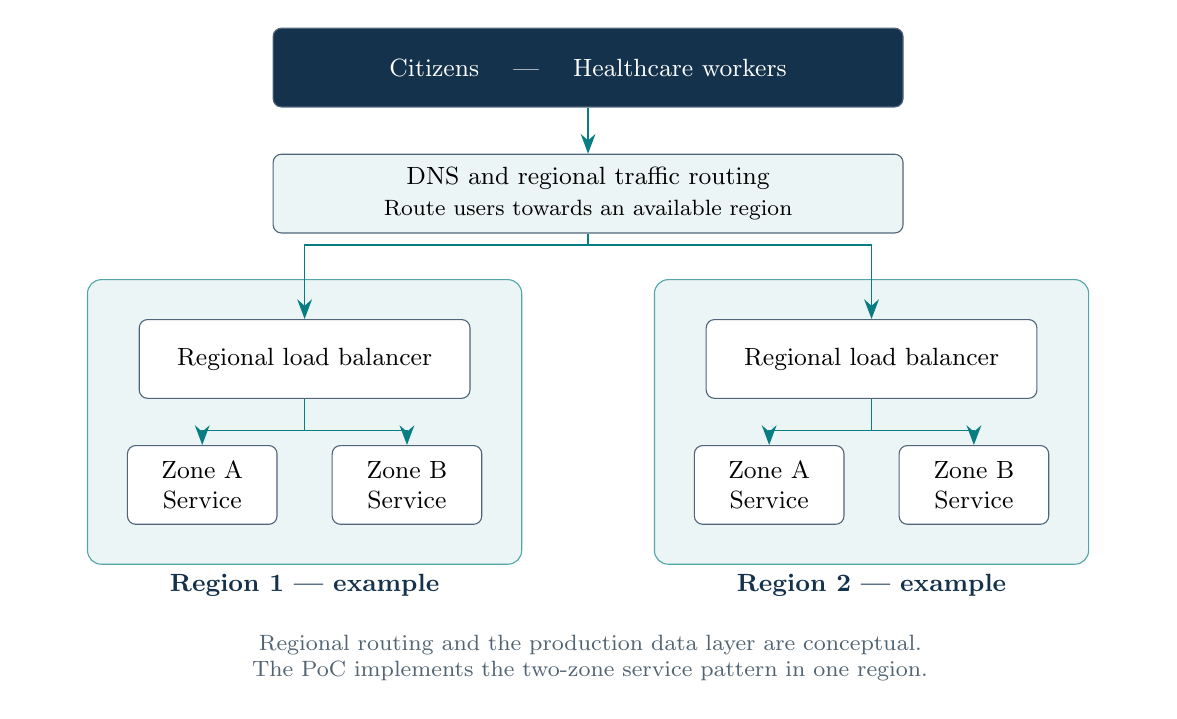
\begin{tikzpicture}[
 font=\small,
 box/.style={draw=navy!75,rounded corners=3pt,fill=white,align=center,minimum height=10mm,minimum width=42mm},
 region/.style={draw=teal!70,rounded corners=5pt,fill=pale,inner sep=5mm},
 flow/.style={-{Stealth[length=2.5mm]},semithick,draw=teal},
 note/.style={font=\footnotesize,align=center,text=graytext}]
\node[box,fill=navy,text=white,minimum width=80mm] (users) at (0,0) {Citizens \quad | \quad Healthcare workers};
\node[box,fill=pale,minimum width=80mm] (route) at (0,-1.6) {DNS and regional traffic routing\\{\footnotesize Route users towards an available region}};
\node[box] (lb1) at (-3.6,-3.7) {Regional load balancer};
\node[box] (lb2) at (3.6,-3.7) {Regional load balancer};
\node[box,minimum width=19mm] (a1) at (-4.9,-5.3) {Zone A\\Service};
\node[box,minimum width=19mm] (b1) at (-2.3,-5.3) {Zone B\\Service};
\node[box,minimum width=19mm] (a2) at (2.3,-5.3) {Zone A\\Service};
\node[box,minimum width=19mm] (b2) at (4.9,-5.3) {Zone B\\Service};
\begin{scope}[on background layer]
\node[region,fit=(lb1)(a1)(b1),label={[font=\bfseries\small,text=navy]below:Region 1 --- example}] (r1) {};
\node[region,fit=(lb2)(a2)(b2),label={[font=\bfseries\small,text=navy]below:Region 2 --- example}] (r2) {};
\end{scope}
\draw[flow] (users)--(route);
\draw[flow] (route.south) -- ++(0,-0.15) -| (lb1.north);
\draw[flow] (route.south) -- ++(0,-0.15) -| (lb2.north);
\draw[flow] (lb1.south) -- ++(0,-0.4) -| (a1.north);
\draw[flow] (lb1.south) -- ++(0,-0.4) -| (b1.north);
\draw[flow] (lb2.south) -- ++(0,-0.4) -| (a2.north);
\draw[flow] (lb2.south) -- ++(0,-0.4) -| (b2.north);
\node[note,text width=140mm] at (0,-7.5) {Regional routing and the production data layer are conceptual. The PoC implements the two-zone service pattern in one region.};
\end{tikzpicture}
\end{center}
\newpage
\sectionline{3. Proposed proof of concept}
\textbf{Scope.} The team plans to deploy a simple vaccine-center lookup service on two servers in different availability zones within one AWS region. A load balancer will distribute requests between them. The service will return static sample data; building a complete vaccination platform is outside the exercise.
\begin{center}
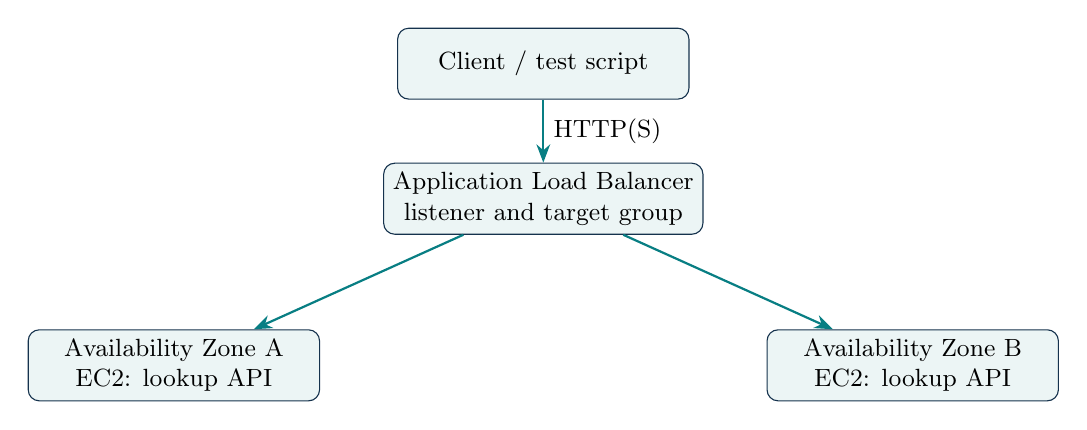
\begin{tikzpicture}[font=\small, node distance=8mm, box/.style={draw=navy,rounded corners,fill=pale,align=center,minimum height=9mm,minimum width=37mm}, arr/.style={-{Stealth},thick,draw=teal}]
\node[box] (client) {Client / test script};
\node[box,below=of client] (alb) {Application Load Balancer\\listener and target group};
\node[box,below left=12mm and 8mm of alb] (a) {Availability Zone A\\EC2: lookup API};
\node[box,below right=12mm and 8mm of alb] (b) {Availability Zone B\\EC2: lookup API};
\draw[arr] (client)--node[right]{HTTP(S)}(alb); \draw[arr] (alb)--(a); \draw[arr] (alb)--(b);
\end{tikzpicture}
\end{center}
\textbf{Purpose.} This scaled-down deployment tests whether the service remains accessible when one server is stopped. The architecture illustrates availability-zone redundancy; it does not implement the multi-region design shown in Section 2.

\textbf{Expected behavior.} When both servers are healthy, the load balancer can route requests to either one. When one server is stopped and detected as unhealthy, requests should be directed to the remaining healthy server. Detection and recovery take time, so the test will record any interruption rather than assume that failover is instantaneous.

\textbf{Final evidence required by the guide.} A national-scale architecture diagram, the working two-zone component, and a video or live demonstration of a server failure and recovery.
\sectionline{4. Implementation and validation plan}
\begin{enumerate}
\item Select an AWS region, instance sizes and a budget; configure a VPC and two availability zones.
\item Deploy the same small API to both instances; confirm the health endpoint works locally.
\item Configure the ALB, listener, target group, security groups and health checks. Record the actual configuration.
\item Establish a baseline by sending repeated requests through the ALB and confirming both targets are healthy.
\item Continue requests while stopping instance A. Record the failure time, target health transition and client-side results.
\item Restore instance A, verify that it becomes healthy, and save screenshots, logs and a video or live demonstration.
\item Clean up resources after evidence collection, subject to the team's submission needs.
\end{enumerate}
\textbf{Measurements.} Record total requests, successful responses, errors, response times and timestamps. Estimate the observed disruption window from the first failed request to the first sustained successful responses, stating the request interval and observation limits. Report the measured outcome even if there is no observed failure. The experiment tests an instance failure, not the loss of an entire availability zone or a full regional disaster.

\newpage
\textbf{Acceptance evidence.} Both targets are initially healthy; a stopped target is marked unhealthy; requests after detection reach the remaining instance; and the team provides a timestamped request log plus AWS health screenshots and a recording. Any failed requests or unexpected behavior will be reported.

\textbf{Cost and operations.} Before deployment, estimate the cost of EC2, the ALB, storage and any data transfer using current regional prices and expected run time. Actual charges depend on account eligibility, resource configuration and usage. Record start and stop times and remove unused resources after the demonstration.

\sectionline{5. Work distribution}
The table assigns proposed ownership. Actual contributions, including infrastructure, research, testing and documentation, will be recorded as work proceeds; they are not limited to GitHub commits.

\small
\begin{tabularx}{\textwidth}{@{}p{31mm}YY@{}}\toprule
\textbf{Member} & \textbf{Week 2: design and planning} & \textbf{Week 3: implementation and evidence}\\\midrule
Jeetrajsinh Gohil\\202303017 & Problem definition, high-availability research, national-scale architecture and report coordination. & Review deployed architecture, help conduct the failover demonstration and document observations.\\\addlinespace
Kaushal Nandaniya\\202303036 & Review Week 1 sources; design AWS topology, resource choices and preliminary cost estimate. & Configure instances, networking, load balancer and health checks; capture infrastructure evidence.\\\addlinespace
Darshil Gandhi\\202301056 & Plan the simple service, failover experiment and evidence collection. & Help build the service and test it; collect logs, screenshots and demonstration evidence.\\\bottomrule
\end{tabularx}
\normalsize
All members will review the report and presentation. The allocation can change based on actual work and availability.
\sectionline{6. References}
\begin{enumerate}[label={[\arabic*]}]
\item Kaushal Nandaniya, \textit{CoWIN: Cloud Platform for COVID-19 Vaccination Scheduling at National Scale}, project repository and Week 1 summary. \href{https://github.com/kaushalnandaniya/CoWIN}{github.com/kaushalnandaniya/CoWIN}.
\item \textit{IT457 Project: Final Deliverables \& Step-by-Step Implementation Guide}, course document, Theme 5: Government and Public Platforms.
\item Instructor clarification shared with the team, 22 October 2026: the exercise is a cloud PoC and contribution may include cloud work beyond code commits.
\end{enumerate}
\end{document}
